\chapter{Einleitung}\label{chapter:einleitung}
%TODO: ADRB2, durchgehend; Skalen; Deckblatt

\section{G-Protein-gekoppelte Rezeptoren (GPCR)}
\label{generalGPCR}
G-Protein-gekoppelte Rezeptoren (GPCRs) stellen die größte Familie der Membranproteine dar. Sie vermitteln zelluläre Antworten auf Hormone und Neurotransmitter, bilden die Rezeptoren des olfaktorischen Systems und können sogar Photonen in zelluläre Signale umsetzen \parencite{Rosenbaum2009}. Allein für das olfaktorische System sind hunderte strukturell verwandter GPCRs bekannt. Damit bilden Moleküle, die GPCRs zum Ziel haben heute die Gruppe der am meisten verwendeten Medikamente \parencite{Pierce2002}.

Alle GPCRs besitzen sieben hydrophobe alpha-helikale Transmembransegmente (7TM-Rezeptoren). Das Aminoende (N-Terminus) ist extrazellulär lokalisiert, das Carboxyende (C-Terminus) intrazellulär. Dazwischen liegen alternierend intra- und extrazelluläre Schleifen. 

Bei beeindruckender funktioneller Diversität lassen sich die GPCRs aufgrund struktureller Homologien in fünf Familien unterteilen \parencite{Fredriksson2003}: Rhodopsin- (Klasse A), Sekretin- (Klasse B), Glutamat- (Klasse C), Adhäsions- (Klasse D) und Frizzled/Taste-Rezeptoren (Klasse E).
Die bei weitem größte unter ihnen bilden die rhodopsinverwandten Rezeptoren (dem "`Lichtrezeptor"' ähnliche Rezeptoren), zu denen auch der in dieser Arbeit näher untersuchte $\beta_2$-adrenerge Rezeptor (ADRB2) gehört.
\subsection{Signaltransduktion}

GPCRs sind in der Lage, stimulatorische (Gs) und inhibitorische guaninnukleotidbindende Proteine (G-Proteine) zu binden, die zu unterschiedlichen Signalkaskaden führen (s. Abb. \ref{fig:gpcr}): 

\begin{figure}[htbp]
	\centering
    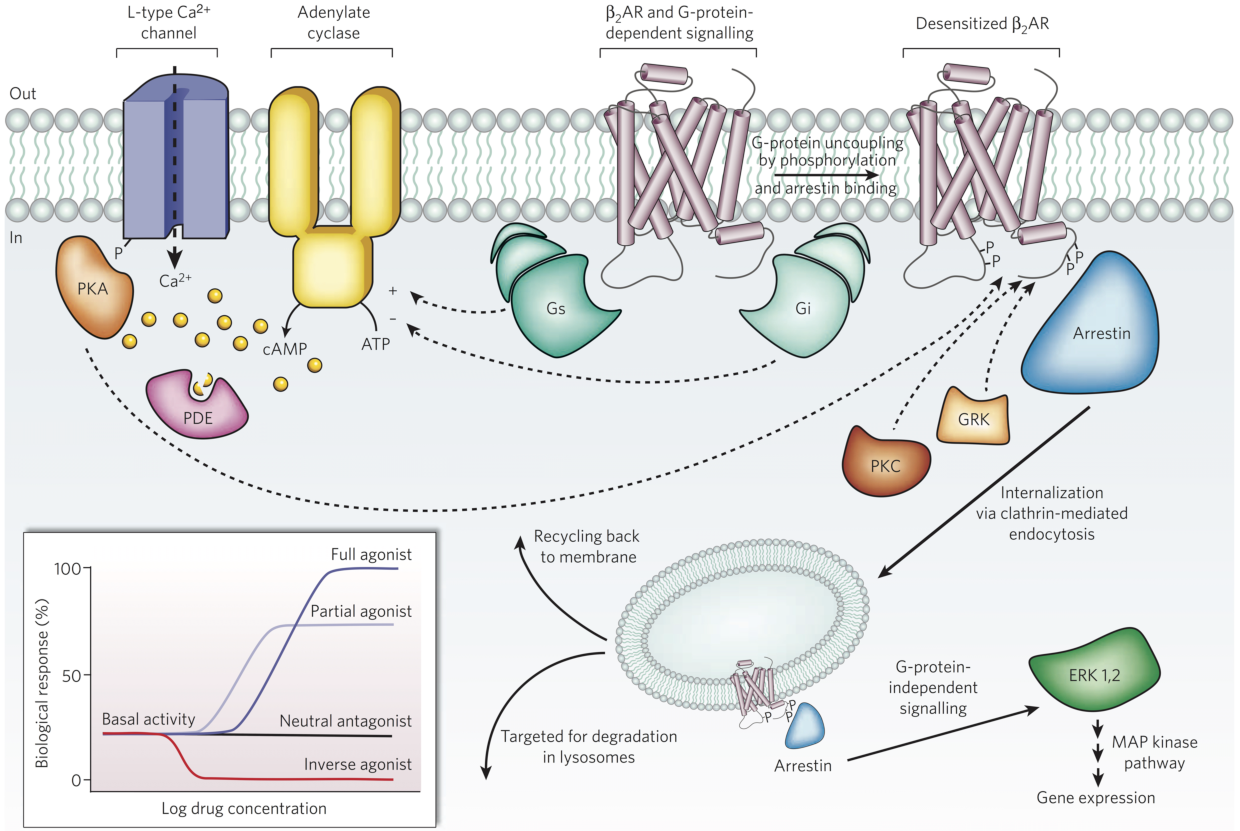
\includegraphics[width=1.0\textwidth]{fig_gpcr.pdf}
    \caption{\textbf{Signaltransduktion eines GPCRs am Beispiel des ADRB2 ($\boldsymbol\beta_2$AR) aus \cite{Rosenbaum2009}}} 
    \label{fig:gpcr}
\end{figure}

Anhand der Funktion des ADRB2 kann die klassische Funktion eines GPCRs illustriert werden: Nach Bindung der natürlichen Agonisten Adrenalin oder Noradrenalin wird die stimulatorische Untereinheit eines heterotrimeren G-Protein aktiviert (G$\alpha$S). Diese führt zur Stimulation der Adenylatzyklase und damit zur Produktion von zyklischem AMP (cAMP). Das akkumulierte cAMP wiederum aktiviert die cAMP-abhängige Proteinkinase A (PKA), die Proteine phosphoryliert und inaktiviert, die für die Kontraktion glatter Muskelzellen verantwortlich sind (L-Typ-Kalziumkanäle) \parencite{Hoffman1982}. 

Die Aktivierung des ADRB2 führt daneben zur Phosphorylierung durch die G-Protein-gekoppelte Rezeptorkinase (GRK). Die Phosphorylierung ermöglicht die Bindung des Proteins Arrestin, das seinerseits als regulatorisches und Signalprotein fungiert. Es deaktiviert den GPCR und führt über Clathrinpits zur endozytotischen Internalisierung des Rezeptors (s. Abschnitt \ref{internalization}), der danach entweder zur Membran recycled oder in Lysosomen degradiert wird. 

Daneben bedingt Arrestin die Aktivierung extrazellulärer signalregulierter Kinasen (ERK 1,2). Diese wiederum regulieren über MAP (mitogen-activated-pathway)-Kinasen die Genexpression.

\section{Adrenerge Rezeptoren}
\subsection{Das $\beta$-adrenerge System}
Die Klasse der adrenergen Rezeptoren umfasst $\alpha$- und $\beta$-adrenerge Rezeptoren. Diese wiederum lassen sich in drei $\alpha_1$-Subtypen ($\alpha_{1A}$, $\alpha_{1B}$, $\alpha_{1D}$), drei $\alpha_2$-Subtypen ($\alpha_{2A}$, $\alpha_{2B}$, $\alpha_{2C}$) sowie in die beiden $\beta$-Subtypen $\beta_1$ und den in dieser Arbeit betrachteten $\beta_2$-Rezeptor unterteilen (\url{http://www.guidetopharmacology.org}).

\subsection{Polymorphismen der $\beta$-adrenergen Rezeptoren}
\subsection{Rezeptorinternalisierung}
\label{internalization}
Gleichzeitig zur Entdeckung, dass durch Agonisten der $\beta$-adrenergen Rezeptoren ein zellulärer  Signalprozess in Gang gesetzt wird, konnten Veränderungen der Rezeptorendichte auf der Membran gefunden werden \parencite{Chuang1979}. 

\section{Oligomerisierung G-Protein-gekoppelter Rezeptoren}
\subsection{Homo- und Heterooligomerisierung G-Protein-gekoppelter Rezeptoren}
Die klassische Annahme, GPCRs würden als monomere Proteine funktionieren, konnte durch eine große Zahl unterschiedlicher Studien widerlegt werden. Tatsächlich sind nach zahlreichen BRET- und FRET-gestützten Untersuchungen mittlerweile sowohl Hetero- als auch als Homodimere einer Vielzahl von GPCRs bekannt (\cite{Khelashvili2010}, \url{http://www.gpcr-okb.org}).

Als Reaktion auf die stetig wachsende Informationen über Rezeptoroligomerisierung veröffentlichte die International Union of Basic and Clinical Pharmacology (IUPHAR) drei Kriterien, von denen mindestens zwei erfüllt sein sollen, um die physiologische Relevanz der Oligomere einordnen zu können \parencite{Pin2007}. Die drei Kriterien umfassen:
\begin{enumerate}
\item Den Nachweis der physischen Interaktion der am Oligomer beteiligten Rezeptoren in nativem Gewebe oder primären Zellen. Dabei wird hinreichende methodische Sicherheit gefordert: Bloße Co-Immunopräzipitationsstudien genügen beispielsweise nicht für den überzeugenden Nachweis physischer Interaktion.
\item Funktionelle oligomerspezifische Besonderheiten wie positive oder negative allosterische Interaktion oder auch den Nachweis eines oligomerspezifischen Liganden (s. Abschnitt \ref{drugs}). Auch der Nachweis einer spezifisch durch den Oligomer modifizierten Signalskaskade kann an dieser Stelle stehen.
\item Validierung des Rezeptoroligomers in-vivo mittels beispielsweise Knock-Out-Mäusen oder RNAi-basierten Methoden - unter der Voraussetzung, dass in heterologen Expressionssystemen bereits hinreichende Relevanz bestätigt werden konnte. 

\end{enumerate}

Zwar ist die Existenz der Rezeptoroligomere in vielen Fällen akzeptiert, doch führt die Bewertung ihrer funktionellen Bedeutung weiter zu kontroversen Diskussionen - etwa weil sich die meisten Untersuchungen heterologer Expressionssysteme bedient haben, die, um Heterooligomere zu untersuchen Rezeptoren exprimierten, die in-vivo nicht gemeinsam exprimiert werden. Zum anderen ist weiter in Diskussion, welche Untereinheiten der Rezeptoren tatsächlich das Interface der beobachteten Rezeptoroligomere bilden \parencite{Terrillon2004}. 

Ebenso bleibt Gegenstand der Diskussion, wie viele Rezeptoren in einem Oligomer gruppiert sind. Häufiger taucht die These auf, Dimere seien die vorherrschende stöchiometrische Einheit \parencite{Dorsch2009}, erst mit steigender Expressionstärke ergäben sich höhergradige Oligomere \parencite{Calebiro2013}. Gleiches konnte für den GABA\textsubscript{B}-Rezeptor beobachtet werden \parencite{Maurel2008, Comps-agrar2011}. Untersuchungen, die sich der Fluorescence-Correlation-Spectroscopy (FCS) und Photon-Counting-Histogram (PCH) bedienen, deuten ebenfalls darauf hin, dass Dimere bei mehreren GPCRs die funktionelle Einheit bilden \parencite{Herrick-Davis2013}. In der vorliegenden Arbeit wird der Begriff "`Oligomere"' bei weiter nicht vollständig geklärter Stöchiometrie bevorzugt, da die wahrscheinliche Dimer-Konfiguration einen Spezialfall des allgemeineren Begriffes darstellt.
\\ \\
Rezeptoroligomere haben eine Reihe denkbarer Implikationen. Fünf postulierte und beobachtete Rollen der Rezeptoroligomerisierung sind in Abbildung \ref{fig:lifecycle} illustriert:

\begin{figure}[htbp]
	\centering
    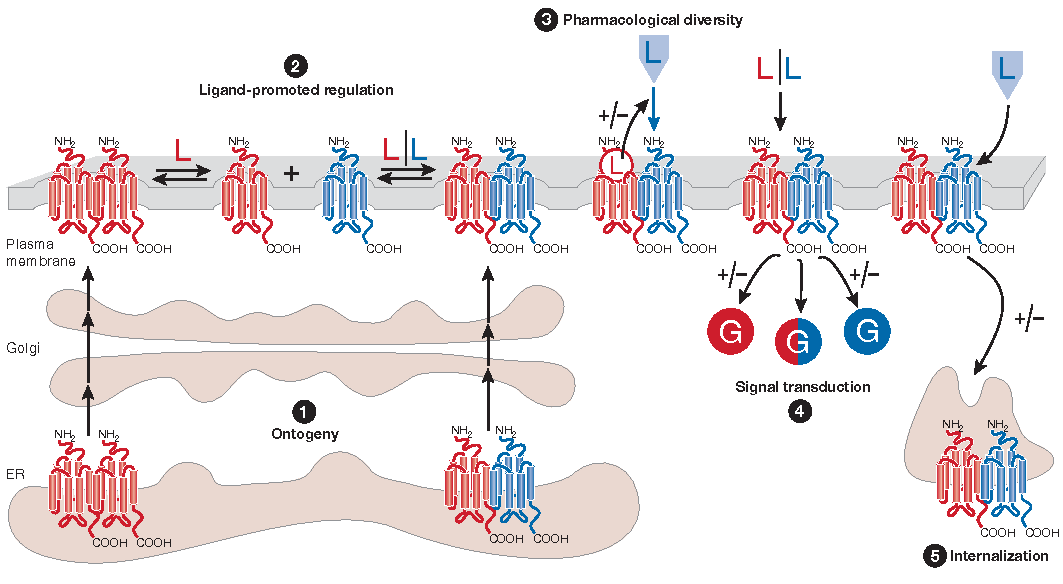
\includegraphics[width=1.0\textwidth]{fig_lifecycle.pdf}
    \caption{\textbf{Rolle der Rezeptoroligomerisierung (aus \cite{Terrillon2004}):} 1 Rezeptorreifung; 2 Dynamische Regulierung der Oligomerisierung durch Ligandenbindung; 3 Heterodimerisierung von Rezeptoren bedingt positiv- oder negativ-kooperative Ligandenbindung; 4 verstärkte und inhibierte Signaltransduktion als Folge der Rezeptoroligomerisierung; 5 Heterooligomerisierung ruft möglicherweise Rezeptorinternalisierung schon bei Aktivierung nur eines Protomers hervor beziehungsweise blockiert ein endozytoseresistenter Protomer die Internalisierung seines gekoppelten Rezeptors im Heterooligomer} 
    \label{fig:lifecycle}
\end{figure}
\begin{itemize}
\item So sind Biosynthese und korrekte posttranslationale Modifikationen im endoplasmatischen Retikulum (ER) möglicherweise Voraussetzung für Integration in die Zellmembran \parencite{Salahpour2004}. Wurden GPCRs mit einem Retentions-Signal versehen, das den Export aus dem Endoplasmatischen Retikulum verhinderte, bedingte dies die Retention des untersuchten Heterooligomers \parencite{Zhu1998, Lee2000, Issafras2002, Floyd2003}.
\item Im Falle des Heterooligomers aus $\mu$- und $\delta$-Opioid-Rezeptoren wurde beobachtet, dass die Bindung eines für den einen Rezeptor spezifischen Liganden über Beeinflussung der Rezeptorkonfirmation die Affinität für den Agonisten des anderen verstärkt \parencite{Gomes2004}. Ein Phänomen, das als positive Kooperativität bezeichnet wird.
\item Auf der Ebene der durch G-Proteine vermittelten Signalkaskade (s. Abschnitt \ref{generalGPCR}) konnte für die Dopaminrezeptoren D1 und D2 im Heterooligomer veränderte Bindungseigenschaften gegenüber dem Gq/11-Protein und somit veränderte Signaleigenschaften gemessen werden \parencite{Rashid2007}.
\item Schließlich konnte gezeigt werden, dass Rezeptorinternalisierung eines Protomers im Fall von Heterooligomeren effektiv auch zur Internalisierung des anderen führen, beziehungsweise diese verhindern kann \parencite{Hillion2002, Milligan2010, Ward2011}. 
\end{itemize}

\subsection{Physiologische Relevanz von Rezeptoroligomeren}
In einer Reihe von Pathologien konnte eine Bedeutung von Rezeptoroligomerisierung im Zusammenhang mit den oben genannten Mechanismen identifiziert werden:
\\ \\
In der Asthmatherapie spielen beispielsweise Agonisten des ADRB2 als Bronchodilatatoren eine führende Rolle. In einer Publikation von \cite{McGraw2006} wurde ein Cross-Talk zwischen dem Prostanoid-Rezeptor EP1 (EP1R) und dem ADRB2 gezeigt: Prostaglandin E2 (PGE2) führte zu verstärkter Dimerisierung des EP1R und des ADRB2 - mit geringerer cAMP-Produktion als Zeichen verminderter ADRB2-Aktivierung.

Bei Patienten mit Major-Depression wurde der Anteil oligomerisierter D1- und D2-Rezeptoren in post-mortem-Studien mittels Co-Immunopräzipitation signifikant erhöht gegenüber gesunden Probanden gemessen \parencite{Pei2010}. Möglicherweise können in Zukunft Medikamente, die die Oligomerisierung der beiden Rezeptoren beeinflussen, therapeutische Bedeutung für die Depression gewinnen. 

In mehreren Untersuchungen, unter anderem mit bivalenten Liganden (s. Abschnitt \ref{drugs}), wurde dem Heterooligomer aus $\delta$- und$\mu$-OR negative Kooperativität in-vivo beigemessen \parencite{Daniels2005, Lenard2007, He2011}. Ähnlich wie bei beim Dopaminrezeptor im Falle der Depression könnte Beeinflussung der Oligomerisierung von pharmakologischer Relevanz werden.
\\ \\
Weitere physiologisch bedeutsame Konstrukte konnten bei der Parkinson-Erkrankung \parencite{Tanganelli2004, Fuxe2003, Fuxe2005} sowie bei Prä-Eklampsie (Hypertonie) \parencite{AbdAlla2001} gefunden werden.

\subsection{Rezeptoroligomere als zukünftiges drug-target}
\label{drugs}
\parencite{George2002, Hiller2013, Ferre2014}
%TODO: incorporate George 2002, Ferré 2014

\section{Methoden zur Untersuchung der Oligomerisierung von Rezeptoren}
\subsection{Überblick}
Es existieren eine Vielzahl von Methoden, die zum Nachweis von Rezeptoroligomerisierung verwendet worden sind. 

\subsubsection {Co-Immunopräzipitation}
Eine der am häufigsten verwendeten Methoden stellt die Co-Immunopräzipitation dar \parencite{Hebert1996, Jordan1999, Hillion2002, Park2004}. In der einfachsten Variante mit einem Protein-Epitop-tag und dem passenden spezifischen Antikörper war aufgefallen, dass die untersuchten Rezeptoren jeweils in den Banden ganzzahliger Vielfacher des Molekulargewichts liefen. Der Vermutung, es könnte sich um Oligomere handeln, liegt nahe. Allerdings konnte so nicht ausgeschlossen werden, dass es sich um unspezifische Rezeptor-Protein-Aggregate handelte. Genauer gelang der Nachweis mithilfe zweier Protein-Epitop-tags und zwei spezifischen Antikörpern. So konnten untersuchte Rezeptoren erst immunpräzipitiert und anschließend mit dem zweiten Antikörper geblottet werden.

\subsubsection{Kristallstrukturen oligomerisierter Rezeptoren}
Eine direkte Nachweismöglichkeit oligomerisierter Rezeptoren bietet die aufwändige Gewinnung der Kristallstruktur der Rezeptoren. Im Falle des CXCR4-Chemokin-Rezeptors und der Opioid-Rezeptor-Subtypen $\mu$OR und $\kappa$OR konnten in den Kristallstrukturen strikte Rezeptordimere beobachtet werden \parencite{Wu2010, Manglik2012, Wu2012}. Die mit dieser Methode identifizierten Oligomerisierungsinterfaces waren für die jeweiligen Rezeptoren unterschiedlich lokalisiert und werden in Zukunft Gegenstand weiterer Analysen werden.

\subsubsection{Fluoreszenz-basierte Methoden}
Fluoreszenz-basierte Methoden zur Analyse der Oligomerstruktur von GPCRs bedienen sich dem Resonanzenergietransfer (RET) zwischen biolumineszenten oder synthetischen Fluorophoren. In Abschnitt \ref{ret} sind die Methoden genauer dargestellt.

\subsubsection{Funktionelle Untersuchungen}

\subsection{BRET \& FRET zur Analyse oligomerisierter Rezeptoren}
\label{ret}
Am häufigsten kommen \gls{bret} und \gls{fret} zum Einsatz. Bei BRET-basierten Analysen werden Fusionsproteine generiert, die C-terminal über ein biolumineszentes Protein, beispielsweise Renilla reniformis Luciferase (Rluc) als Donor und fluoreszente Proteine wie YFP als Akzeptor.

%TODO:RET-acro
\subsection{Proteinlabeling mit dem SNAP-tag}
Zur spezifischen Adressierung von Proteinen wie den GPCRs existieren eine Reihe unterschiedlicher Systeme. Neben Verfahren, die sich auf strukturell große Antikörper stützen können tag-Systeme mit intrinsischer Aktivität verwendet werden, um spezifische kovalente mit den gewünschten Proteinuntereinheiten zu katalysieren \parencite{Gautier2008}.
\subsection{time-resolved FRET}

\section{Zielsetzung dieser Arbeit}